%
% $XORP: xorp/docs/multicast/multicast_arch.tex,v 1.21 2007/03/14 00:20:35 pavlin Exp $
%

\documentclass[11pt]{article}

%\usepackage[dvips]{changebar}

\usepackage{subfigure}
\usepackage{fullpage}
\usepackage{setspace}
\usepackage{times}
\usepackage{latexsym}
\usepackage{epsfig}
\usepackage{graphicx}
\usepackage{xspace}
\usepackage{color}
\usepackage{amsmath}
\usepackage{rotating}
\usepackage{moreverb}
\usepackage{listings}
\usepackage{alltt}
\usepackage{stmaryrd}
%\usepackage[dvipdf]{graphics}
%\usepackage[dvips]{graphicx}
%\usepackage{xorp}

\definecolor{gray}{rgb}{0.5,0.5,0.5}
\newcommand{\etc}{\emph{etc.}\xspace}
\newcommand{\ie}{\emph{i.e.,}\xspace}
\newcommand{\eg}{\emph{e.g.,}\xspace}
%\newcommand{\comment}[1]{{\color{gray}[\textsf{#1}]}}
%\newcommand{\comment}[1]{}

% Changebar stuff
% \newenvironment{colorcode}{\color{blue}}{}
% \renewcommand{\cbstart}{\begin{colorcode}}
% \renewcommand{\cbend}{\end{colorcode}}

% \pagestyle{empty}

\begin{document}

\title{XORP Multicast Routing Design Architecture \\
\vspace{1ex}
Version 1.4}
\author{ XORP Project					\\
	 International Computer Science Institute	\\
	 Berkeley, CA 94704, USA			\\
         {\it http://www.xorp.org/}			\\
	 {\it feedback@xorp.org}
}
\date{March 20, 2007}

\maketitle


%%%%%%%%%%%%%%%%%%%%%%%%%%%%%%%%%%%%%%%%%%%%%%%%%%%%%%%%%%%%%%%%%%%%%%%
\section{Introduction}


%%%%%%%%%%%%%%%%%%%%%%%%%%%%%%%%%%%%%%%%%%%
\subsection{Overview}

This document provides an overview of the XORP multicast routing
architecture.  It is intended to provide a starting point for software
developers who wish to modify the multicast-related software.

The XORP multicast architecture consists of user-level software
implementation of multicast routing protocols such as PIM-SM and IGMP.
This document provides an overview of the interaction among them,
as well as the interaction with the underlying multicast forwarding
engine and other parts of the system.

As with the other parts of the XORP architecture, the multicast
architecture is based on modularity and abstraction.
In particular, there is one process per protocol, and each process
typically communicates with other processes by using XRLs, the XORP
inter-process communication mechanism~\cite{xorp:xrl}.

%%%%%%%%%%%%%%%%%%%%%%%%%%%%%%%%%%%%%%%%%%%
\subsection{Acronyms}

Acronyms used in this document:

\begin{itemize}

  \item {\bf FEA}: {\bf F}orwarding {\bf E}ngine {\bf A}bstraction

  \item {\bf FIB}: {\bf F}orwarding {\bf I}nformation {\bf B}ase

  \item {\bf MFC}: {\bf M}ulticast {\bf F}orwarding {\bf C}ache: another
  name for an entry in the multicast forwarding engine (typically used
  on UNIX systems).

  \item {\bf MFEA}: {\bf M}ulticast {\bf F}orwarding {\bf E}ngine
  {\bf A}bstraction

  \item {\bf MLD/IGMP}: {\bf M}ulticast {\bf L}istener {\bf D}iscovery/{\bf
  I}nternet {\bf G}roup {\bf M}anagement {\bf P}rotocol

  \item {\bf MRIB}: {\bf M}ulticast {\bf R}outing {\bf I}nformation
  {\bf B}ase

  \item {\bf PIM-SM}: {\bf P}rotocol {\bf I}ndependent {\bf M}ulticast--{\bf
  S}parse {\bf M}ode

  \item {\bf RIB}: {\bf R}outing {\bf I}nformation {\bf B}ase

\end{itemize}


%%%%%%%%%%%%%%%%%%%%%%%%%%%%%%%%%%%%%%%%%%%%%%%%%%%%%%%%%%%%%%%%%%%%%%%
\section{Protocol Abstraction}

As with the rest of the XORP architecture, the XORP multicast routing
architecture is designed such that each of the implemented protocols
can be used for both real-world routing and for network simulations.  A
simulation can be composed of several (UNIX) processes, one per
protocol entity controlled by a single process, or all protocol entities
running within a single process. For debugging purpose the latter may be
simpler to use and control. Further, the all-in-one model might be more
scalable. The implication of this is that a protocol implementation
must not keep any global state.

In routing, the concept of a network port or interface is essential in a
sense that a routing protocol entity communicates with the rest of the
world through such ports/interfaces (think of this as a protocol entity
having several virtual interfaces and each virtual interface corresponds
to a physical interface, and those interfaces are used for
sending/receiving control messages to/from other routers). In case of
PIM for example, the routing entity has several virtual interfaces one
per each physical interface it controls.  In case of BGP,
the routing entity has several ports, one per each BGP peering.

In term of C++ implementation, each virtual interface is a class; each
protocol entity is a separate class: a single protocol object has several
virtual interfaces (see Figure~\ref{fig:mcast_proto_abstraction}).

\begin{figure}[htbp]
  \begin{center}
    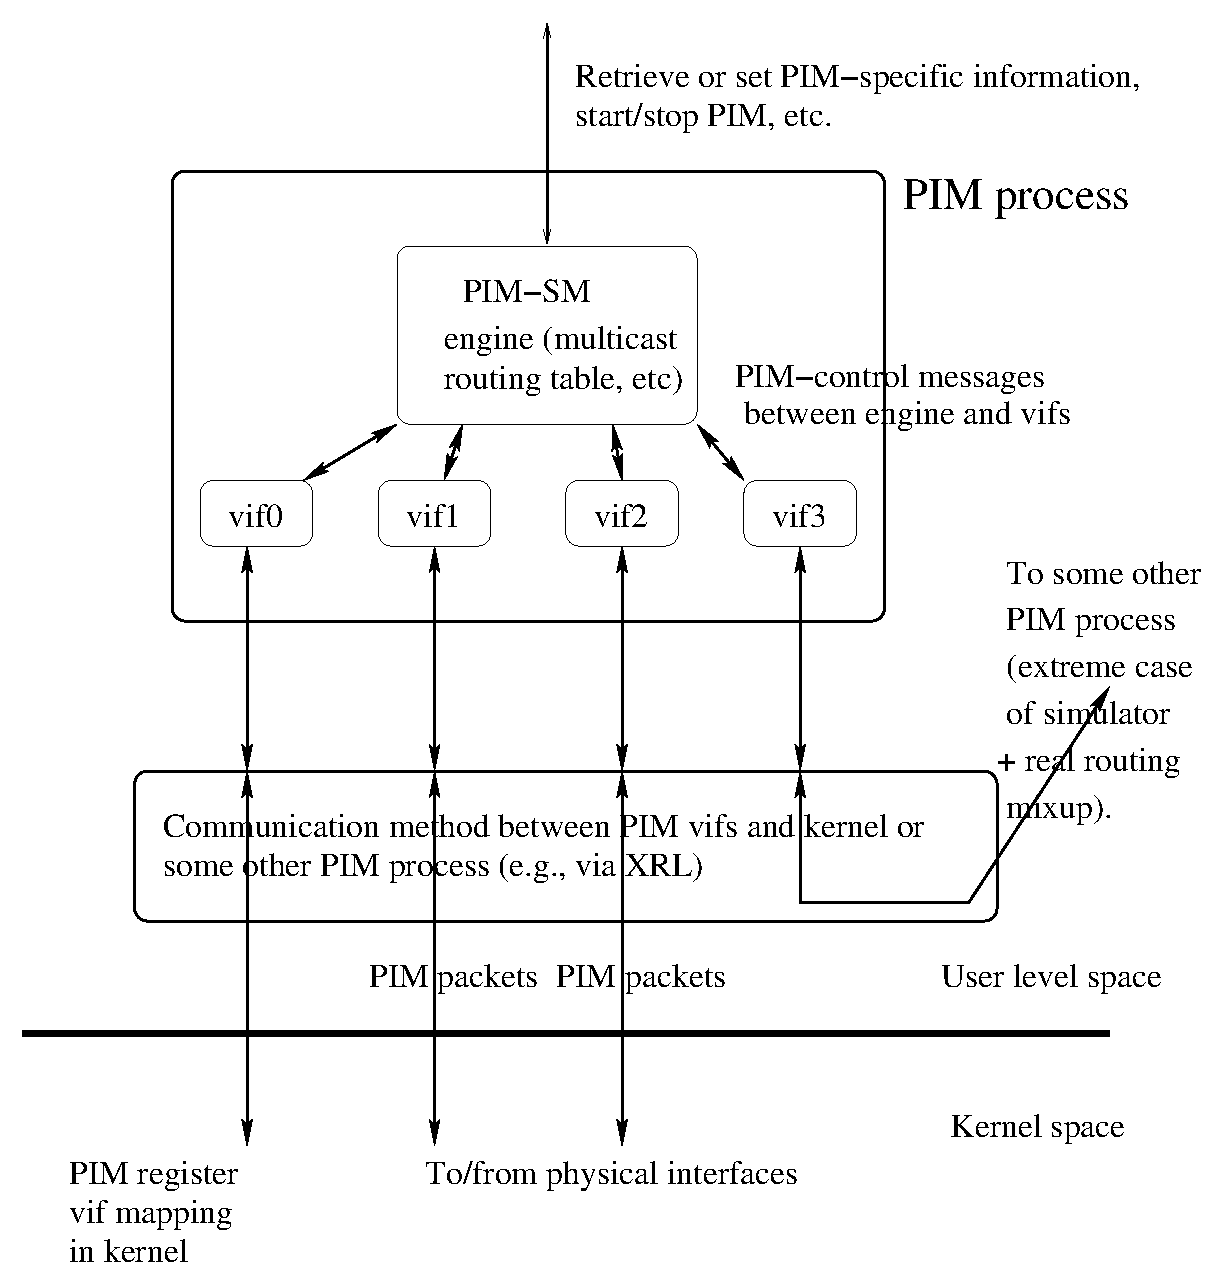
\includegraphics[width=5.0in]{figs/mcast_proto_abstraction}
    \caption{Multicast protocol abstraction}
    \label{fig:mcast_proto_abstraction}
  \end{center}
\end{figure}

At the protocol level implementation, the virtual interfaces do not
posses knowledge about the particular communication method used to send
or receive packets. To achieve this, the implementation uses pure
virtual C++ class methods (\eg methods declared such as:
{\it virtual int send() = 0;}).
The declaration of such methods requires that each class must be
inherited by a ``wrapper'' class that implements all pure virtual
methods. Then, all the details about the particular mechanism
that is used to send or receive packets are in this wrapper class.
For example, that class might use XRLs, but it could be any other
mechanism that the developer provides (\eg a third-party simulation
testbed environment).

Such abstraction makes it very easy to reuse the protocol-specific code
for any other purpose, or to create several virtual ``nodes'' each of
them running the particular protocol. Those nodes can be either within
the same (UNIX) process or each of them running as a separate process,
as long as we have the right mechanism that allows them to communicate
with each other.

%%%%%%%%%%%%%%%%%%%%%%%%%%%%%%%%%%%%%%%%%%%%%%%%%%%%%%%%%%%%%%%%%%%%%%%
\section{MLD/IGMP Daemon/Library}

A physical interface is owned by a single multicast routing
protocol, therefore we can have MLD/IGMP running as a library linked with
a multicast routing protocol on each of the
interfaces owned by that protocol. This solution may not work only if
there is more than one protocol that needs multicast group membership
information on an interface.

The alternative solution is to have a separate MLD/IGMP daemon that
takes care of multicast group membership for all interfaces, and then
reports that information to all interested parties. Thus, more than one
protocol may receive multicast group membership information per
interface.

Separating MLD/IGMP from the routing code has the advantage of reducing
dependency and improving robustness; \eg if the MLD/IGMP code crashes, the
routing protocol can continue running. Further, if we want to upgrade
the software, and if we are running MLD/IGMP as a
separate process, then the upgrade can be performed by starting a new
MLD/IGMP daemon in place of the old one. Therefore, the upgrade does
not require to stop the PIM daemon for example, which is very important
for routers in real-world operation.

%%%%%%%%%%%%%%%%%%%%%%%%%%%%%%%%%%%%%%%%%%%%%%%%%%%%%%%%%%%%%%%%%%%%%%%
\section{Multicast Modules Interaction}

\begin{figure}[htbp]
  \begin{center}
    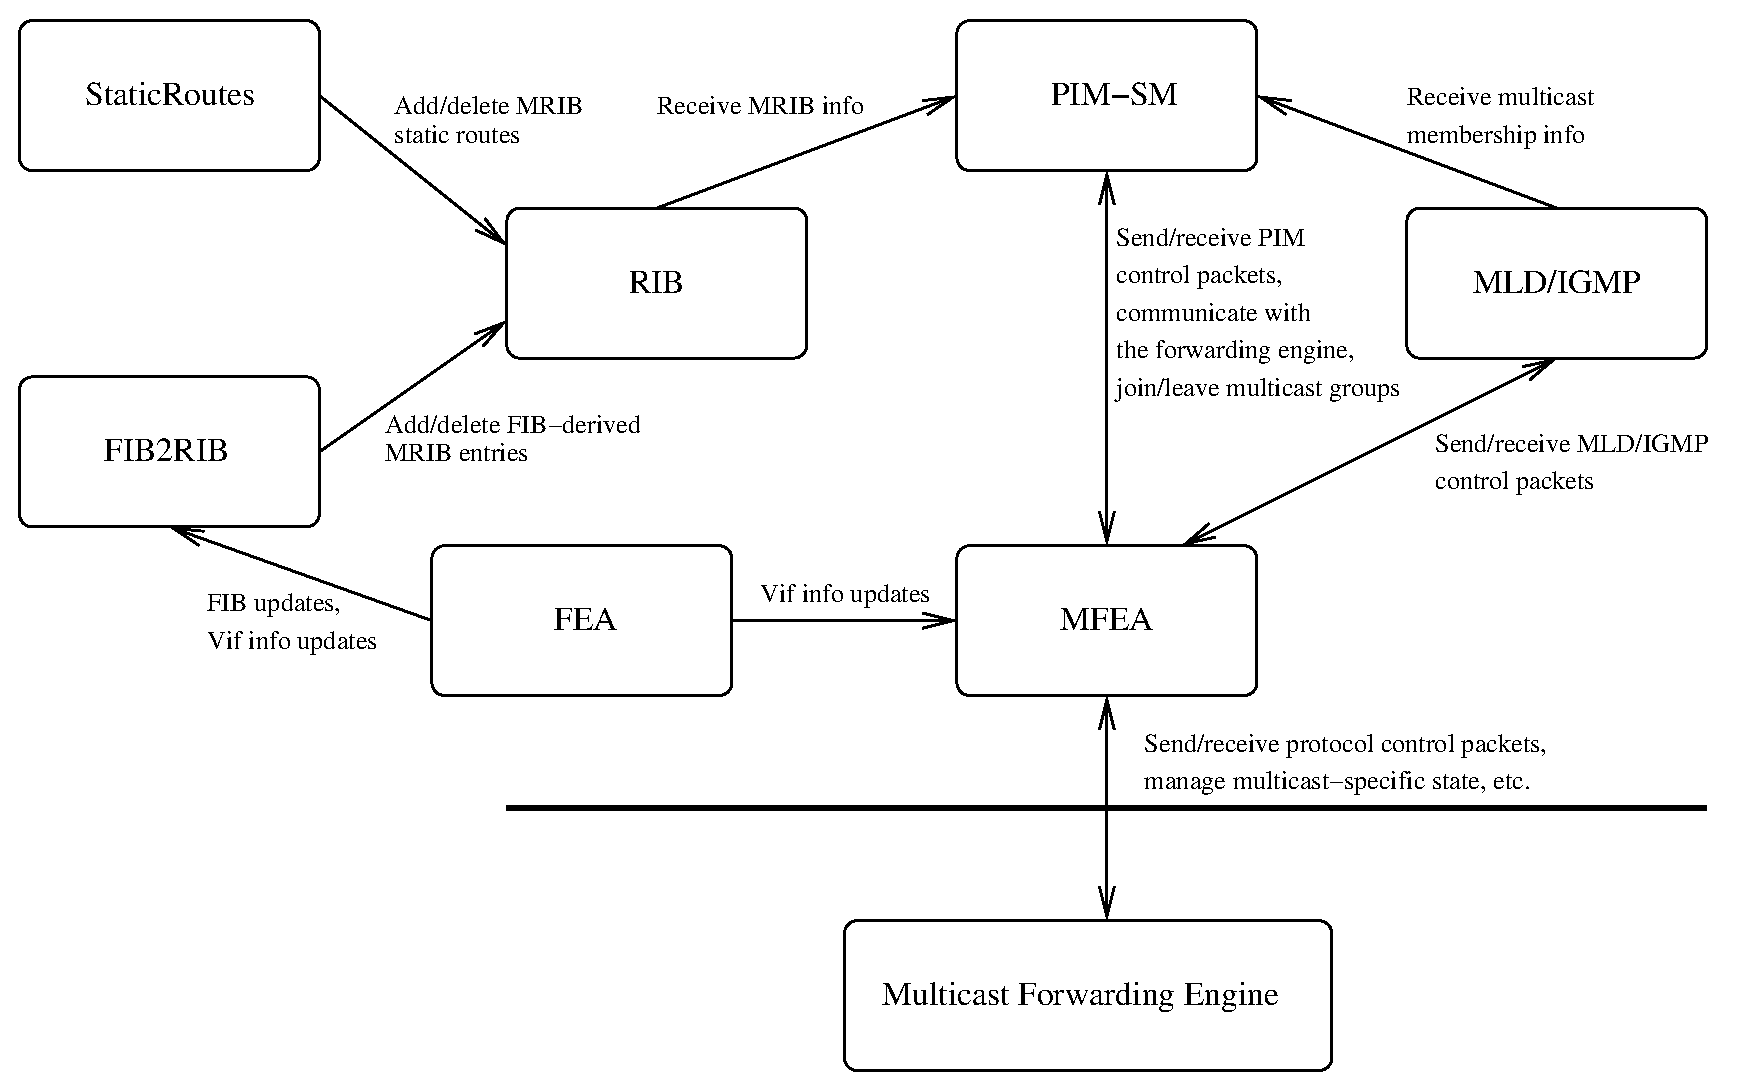
\includegraphics[scale=0.5]{figs/mcast_modules_interaction}
    \caption{Multicast Modules Interaction}
    \label{fig:mcast_modules_interaction}
  \end{center}
\end{figure}

Figure~\ref{fig:mcast_modules_interaction} shows the interactions between
the multicast-related modules. Those interactions are:

\begin{itemize}

  \item FEA--MFEA: to propagate vif-related information updates from the
   FEA to the MFEA.

  \item MFEA--PIM: to send or receive PIM control packets, to forward
   PIM-related signals from the multicast forwarding engine to PIM, to
   establish the communication between PIM and the multicast-forwarding
   engine, for the MFEA to join or leave a multicast group on behalf of
   PIM, etc.

  \item MFEA--MLD/IGMP: to send or receive MLD/IGMP control
  packets, and to join or leave a multicast group on behalf of
  MLD/IGMP.

  \item MLD/IGMP--PIM: for PIM to monitor multicast membership about
  local members.

  \item RIB--PIM: for PIM to obtain MRIB information.

  \item FEA--FIB2MRIB: to propagate the FIB updates to the FIB2MRIB module.

  \item FIB2MRIB--RIB: to add/delete FIB-derived MRIB entries.

  \item StaticRoutes--RIB: to add/delete MRIB-specific static routes.

\end{itemize}

In the next subsections we describe those interactions.

%%%%%%%%%%%%%%%%%%%%%%%%%%%%%%%%%%%%%%%%%%%
\subsection{Interaction between the FEA and MFEA modules}

The MFEA module needs to interact with the FEA module to obtain the
vif-related information, and to keep track if there is any change.
If there is any change in the vif information, the MFEA saves that
information locally and propagates it to the modules that have
registered interest with the MFEA (\eg MLD/IGMP and PIM-SM).

%%%%%%%%%%%%%%%%%%%%%%%%%%%%%%%%%%%%%%%%%%%
\subsection{Interaction between the MFEA and PIM modules}

PIM-SM needs to interact with the MFEA module for the following:

\begin{itemize}

  \item Send PIM control packets to other PIM routers, and receive PIM
  control packets from them.

  \item Start/stop the multicast forwarding engine.

  \item Add/delete multicast interface in the multicast forwarding
  engine.

  \item Add/delete multicast forwarding entry in the multicast
  forwarding engine.

  \item Receive PIM-related signals from the multicast forwarding engine
  (when applicable). Examples of such signals in case of UNIX kernel are
  NOCACHE or WRONGVIF/WRONGMIF: the former one is sent when the
  underlying multicast
  forwarding engine has no multicast forwarding entry for a multicast
  packet; the latter one is sent when a multicast data packet has
  arrived on an interface that is not the expected incoming interface to
  forward that data packet.

  \item Receive bandwidth-related information about multicast data
  flows: \eg whether a data flow is idle, or whether the bandwidth of a
  data flow is above a pre-defined threshold (needed by PIM-SM to perform
  bandwidth-based Shortest-Path switch toward a source).

  \item Join/leave a multicast group.

  \item Obtain information about existing interfaces on a router.

\end{itemize}

On startup, the PIM module registers with the MFEA. As part of this
registration, the MFEA sends information about existing
interfaces on the system, and the current unicast forwarding
information. If any of this information changes later, the MFEA sends
the appropriate update to PIM. In addition, the MFEA creates the
appropriate state to send and receive PIM control packets. After the
PIM module receives the network interface information, it instructs the
MFEA to start PIM operation on selected interfaces. After that the PIM
module can send and receive PIM control packets on those interfaces.
Also, it can send requests to the MFEA to add, delete or modify multicast
forwarding entries in the kernel.

Note that the default solution in case of UNIX PIM kernel
uses one more signal from the kernel to the user-level daemon:
{\emph WHOLEPKT} messages. Those messages are multicast packets that are
suppose to be encapsulated in a PIM-SM Register message and sent to the
RP. The encapsulation mechanism must know the RP address (in general,
per multicast group address), threfore to avoid putting the RP addresses in
the kernel (which would also change the traditional UNIX multicast API), the
default solution is to use user-level encapsulation.  To improve
performance, the PIM encapsulation should be done in the kernel, and
then we need a signaling mechanism between the kernel and the user
process managing the kernel multicast forwarding entries. That mechanism
would deal with installing the appropriate information needed by kernel-level
Register encapsulation. Currently (March 2007), only recent releases
of DragonFlyBSD, FreeBSD, NetBSD, and OpenBSD do support such
kernel-level encapsulation.

%%%%%%%%%%%%%%%%%%%%%%%%%%%%%%%%%%%%%%%%%%%
\subsection{Interaction between the MFEA and MLD/IGMP modules}

MLD/IGMP needs to interact with the MFEA module for the following:

\begin{itemize}

  \item Send and receive MLD/IGMP control messages.

  \item Join/leave a multicast group.

  \item Obtain information about existing interfaces on a router.

\end{itemize}

On startup, the MLD/IGMP module registers with the MFEA. As part of this
registration, the MFEA sends information about existing
interfaces on the system. If
any of this information changes later, the MFEA sends the appropriate update
to MLD/IGMP. In addition, the MFEA creates the appropriate state to send and
receive MLD/IGMP control packets. After the MLD/IGMP module receives the
network interface information, it instructs the MFEA to start MLD/IGMP
operation on selected interfaces. After that the MLD/IGMP module can send and
receive MLD/IGMP control packets on those interfaces.

%%%%%%%%%%%%%%%%%%%%%%%%%%%%%%%%%%%%%%%%%%%
\subsection{Interaction between the MLD/IGMP and PIM modules}

PIM-SM needs to interact with the MLD/IGMP module to receive multicast
membership information about local members. On startup, the PIM module
registers with the MLD/IGMP module by expressing interest in tracking
multicast membership on selected network interfaces. After that, if
the multicast membership on any of the selected interfaces changes, the
MLD/IGMP module informs the PIM module about the change: \eg ``add
membership for group 224.0.1.20 on interface vif0''.

Note that control packets used for multicast debugging such as MRINFO or
multicast traceroute use IGMP as the network protocol. Hence, if such
messages are received by the MLD/IGMP module, the appropriate
information should be sent to the PIM module. Currently (March 2007),
the handling of such messages is not implemented yet.

%%%%%%%%%%%%%%%%%%%%%%%%%%%%%%%%%%%%%%%%%%%
\subsection{Interaction between the RIB and PIM modules}

The PIM module needs to interact with the RIB module to obtain the MRIB
information, and to keep track if there is any change.

%%%%%%%%%%%%%%%%%%%%%%%%%%%%%%%%%%%%%%%%%%%
\subsection{Interaction between the FEA and FIB2MRIB modules}
\label{sec:fea-to-fib2mrib-interaction}

Typically, the MRIB information inside the RIB module will be populated by
entries from the unicast routing protocols running as part of a XORP
router. For example, if Multiprotocol BGP is running on the system, it can be
used to supply routes that are multicast-only; those routes then will be
stored in the MRIB. However, if a XORP router is used only for multicast
routing, and if there are no XORP unicast routing protocols to supply the MRIB
routes, then by default we would use the existing unicast forwarding
entries from the FIB in the underlying system. Those entries may have been
statically installed on system startup, or may be managed by a non-XORP
unicast routing implementation.

The FIB2MRIB module is used to receive the FIB updates from the FEA.
It also receives network interface related information from the FEA.
The FIB information is updated by the network interface related information,
(e.g., FIB entries that use disabled interfaces are withdrawn),
and the result is propagated as MRIB entries to the RIB module.

%%%%%%%%%%%%%%%%%%%%%%%%%%%%%%%%%%%%%%%%%%%
\subsection{Interaction between the FIB2MRIB and the RIB modules}

See Section~\ref{sec:fea-to-fib2mrib-interaction}.

%%%%%%%%%%%%%%%%%%%%%%%%%%%%%%%%%%%%%%%%%%%
\subsection{Interaction between the StaticRoutes and the RIB modules}

The StaticRoutes module is used to store and manipulate the static unicast and
multicast routes. A configured static route is added directly to the
StaticRoutes module. This information is updated by the network interface
related information obtained from the FEA (not shown on
Figure~\ref{fig:mcast_modules_interaction}). For example, static routes
that use disabled interfaces are withdrawn. The result is propagated
as URIB or MRIB entries to the RIB module.


%%%%%%%%%%%%%%%%%%%%%%%%%%%%%%%%%%%%%%%%%%%%%%%%%%%%%%%%%%%%%%%%%%%%%%%
%     APPENDIX
%%%%%%%%%%%%%%%%%%%%%%%%%%%%%%%%%%%%%%%%%%%%%%%%%%%%%%%%%%%%%%%%%%%%%%%
\appendix
\section{Modification History}

\begin{itemize}

  \item December 11, 2002: Initial version 0.1 completed.

  \item March 10, 2003: Updated to match XORP release 0.2.

  \item June 9, 2003: Updated to match XORP release 0.3:
  changes related to the MFEA--FEA merging.

  \item August 28, 2003: Minor cleanup.
  Updated the version to 0.4, and the date.

  \item November 6, 2003: Minor cleanup.
  Updated the version to 0.5, and the date.

  \item July 8, 2004: Updated to match XORP release 1.0: added information
  about the FIB2MRIB and StaticRoutes modules.

  \item January 27, 2005: Removed MFEA+MRIB-related text, because the MFEA
  does not deal with the MRIB information anymore.

  \item April 13, 2005: Updated the list of the OS-es that support
  kernel-level PIM Register encapsulation.
  Updated the version to 1.1, and the date.

  \item March 8, 2006: Updated the version to 1.2, and the date.

  \item August 2, 2006: Updated the version to 1.3, and the date.

  \item March 20, 2007: Updated the version to 1.4, and the date.

\end{itemize}


%%%%%%%%%%%%%%%%%%%%%%%%%%%%%%%%%%%%%%%%%%%%%%%%%%%%%%%%%%%%%%%%%%%%%%%
%     BIBLIOGRAPHY
%%%%%%%%%%%%%%%%%%%%%%%%%%%%%%%%%%%%%%%%%%%%%%%%%%%%%%%%%%%%%%%%%%%%%%%
\bibliography{../tex/xorp}
\bibliographystyle{plain}

%%%%%%%%%%%%%%%%%%%%%%%%%%%%%%%%%%%%%%%%%%%%%%%%%%%%%%%%%%%%%%%%%%%%%%%
\end{document}
